%!TEX root = ../dissertation.tex
\chapter{Amortization: Memory as a computational resource}
\label{chap:amort}

%Tie in AI refs, expand ecological rationality idea with LTI figure perhaps.

In this chapter, I introduce the concept of \textit{amortization}. The word refers more generally to the concept of spreading costs over a period of time. In our case, these are computational costs that can be amortized by re-using parts of previously computed solutions. Therefore, simply by remembering past solutions to problems, and flexibly re-using them in the face of new problems, we can use memory as a computational resource to ease the burden of real-time computation to solve new problems. 

In this chapter, I will first discuss the computational problem that amortization addresses. I then discuss how it links to ecological rationality, as well as outline how it might be implemented. Finally, I discuss amortization in models of human cognition.

\section{Two kinds of knowledge}

There are two distinct aspects to making an inference. The first is the have the relevant information from the external world that will best inform that inference. In the context of the domains this thesis concerns, this means having a good (structured, probabilistic) generative model for how that aspect of the world works, either from previous experience, or through instruction, or in the case of artificial systems by explicitly encoding this information. Once a system has this information, it is in theory possible to make normative inferences within this model. But these normative inferences remain to be computed from this information. The second aspect therefore is to actually perform the computations that result in an inference: compiling abstract understanding of the world in the form of a model to an actual response. We refer to the first kind of information as `potential knowledge', since all optimal inferences are in theory possible to compute, once we have an accurate model of how the world works. We refer to information obtained by actually computing inferences in such a model as `realized knowledge'. 

We give an example for intuition. Once we learn the rules of mathematics, the proofs of all the theorems in the world are included in potential knowledge. However, only a small subset of these proofs can and will actually be computed by anyone who knows the rules of mathematics. This subset is realized knowledge. Arriving at each of these proofs requires some work. Even if we already know enough about a domain works, suggesting that all potential knowledge is within reach, going from that to realized knowledge can require prohibitive amounts of computation. These computations cost resources. It is these costs that we wish to amortize. 

Since we are concerned primarily with the computations involved in going from potential to realized knowledge, we often assume that potential knowledge has already been acquired and what remains is to compute realized knowledge. All of the experiments and models in this thesis concerning human cognition assume that people have already acquired potential knowledge, and we primarily discuss how the costs of going from potential to realized knowledge (i.e. actually making inferences in a provided probabilistic model) might be amortized, leading to ecologically rational behavior. In our discussions of artificial intelligence, the line between realized and potential knowledge can be more blurred. We discuss this later in this chapter, as well as include a broader discussion of these two kinds of knowledge in the Conclusion (Chapter \ref{chap:conclusion}).

\section{Amortization and ecological rationality}

As mentioned earlier, we assume for now that we already know how the world works, and all potential knowledge is within reach. When faced with a new query, the challenge is in performing the computations that go from this potential knowledge to an (approximately) optimal response to this query. This might require extensive computational resources. If there is structure in the space of queries observed -- such that similar queries appear often, or certain parts of the hypothesis space are never queried -- then it is wasteful to not leverage this structure and instead simply recompute responses to each query independently every time it is encountered. The challenge then is to know when and how to re-use parts of previously computed responses. This amounts to amortizing the costs of computing a response to a query over many previously encountered similar queries, and using memory as a means for easing the burden of computation.

Amortizing the costs of computation is `rational' only if there exists structure in the environment  such that we expect some similarity in queries encountered. This is guaranteed in any domain with finite hypotheses and infinite experienced queries, but will be more prevalent in certain domains than others. In different environments, with different distributions of queries, different levels of amortization can be optimal. For example, if a query is rarely experienced, there may not exist adequate previous experience to re-use. Further, the cost of storing and recovering previous solutions might not be worth the computational savings incurred from amortization -- especially if the possibility of it being encountered again is rare. However, when we have a large amount of experience in an environment, and there does exist some additional structure in the space of queries, it becomes more rational to amortize computations. These are the domains we focus on
%\footnote{Some of our experiments are carried out in artificial environments where it is unclear if these properties hold. But we see that inference strategies developed over everyday experience in a world where such structure exists, result in amortization even in artificial environments.}
, and argue that the re-use of computations in such structured environments can lead to ecological rational behavior -- i.e. behavior that adapts to and exploits structural regularities in an environment. 

\begin{figure}
\centering
  \subfloat[True posterior, overlaid with query distribution]{% 
      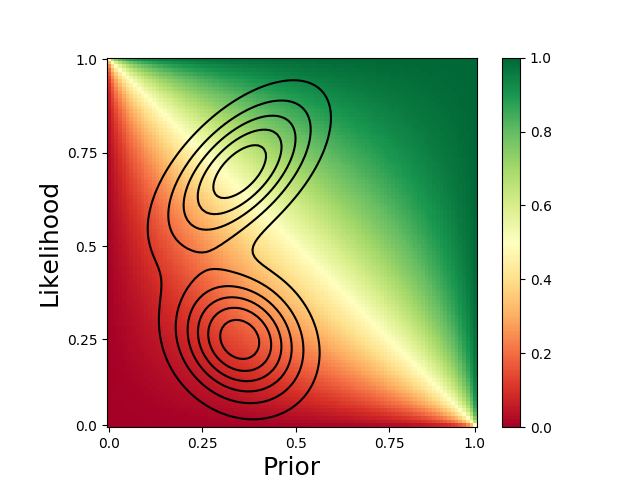
\includegraphics[width=0.48\textwidth]{Figures/all_posts.png}} 
  \subfloat[Amortized values for queries]{% 
    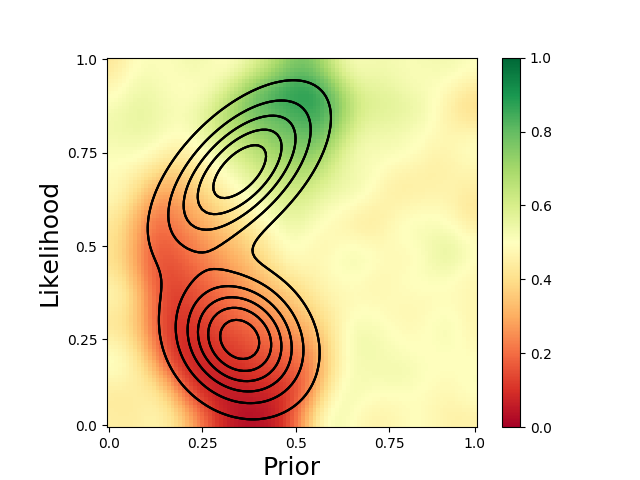
\includegraphics[width=0.48\textwidth]{Figures/all_finalQs.png}} 
  \caption{\textbf{Schematic demonstration of amortizing past queries}. (A) The true posterior probability (indicated by colors on the heatmap), as a function of the prior and likelihood for a generative model in which $h \sim \text{Bernoulli}(p_0)$ and $d|h \sim \text{Bernoulli}(p_l)$. The contour lines depict the query distribution. (B) Amortized estimates based on previously encountered queries (indicated by colors on the heatmap) are possible and reliable only in the space of frequently encountered queries (as depicted by contour lines).} 
  \label{fig:ecol_ration_schematic}
\end{figure}

We expand on the technical aspects of this adaptation, and formalize it more broadly in greater detail in Chapter \ref{chap:LTI}, but Figure \ref{fig:ecol_ration_schematic} provides some intuition for how environment sensitivity arises when amortizing computations. First, we see that good amortized estimates are only possible for frequent queries. In Figure \ref{fig:ecol_ration_schematic}(b), we see that the other queries for which the amortized approximation follows the true probability distribution well are for queries that have been observed (depicted by contour lines). This could explain context-sensitivity in why people are so close to optimal for certain queries in certain domains, but exhibit inferential errors in others, despite similar run-time computational resources in both. Second, we see that there might be underlying, lower dimensional structure in the space of frequently observed queries, that allows effective heuristic strategies. In the example shown, we see that the variance in the prior probability in the space of observed queries (the contour lines) is much lower than the variance in the likelihood. Within the distribution of these observed queries, a heuristic that only attends to the likelihood would perform reasonably well. In Figure \ref{fig:ecol_ration_schematic}(b), we see that `high likelihood implies high posterior' and similarly for low likelihoods, roughly holds. This same heuristic however does not perform well in general in this domain, and would fail on queries that come from outside the depicted query distribution. This explains the emergence of context-sensitive, ecologically rational heuristic inference.

This mechanism for the arisal of ecological rationality addresses some of the concerns raised in Chapter \ref{chap:psych} about how ecologically rational behavior might come about. To briefly re-iterate the concern, while heuristic behavior in humans has been characterized ecologically rational\cite{gigerenzer2008heuristics}, they largely remain `as-if' models -- that show that the heuristics implemented in human inference are `as-if' humans are implementing ecological rational shortcuts. But it remains to be understood how these heuristics arise, and further, how one chooses the right heuristic for the right environment -- with the computations required to make this choice often being comparably expensive to computing the optimal response from scratch\cite{hay2014selecting, horvitz1989reflection}. The mechanism of simply reusing the procedures that worked well for previously encountered queries in an environment, by amortizing the computations that go into computing these responses, allows for a feasible way to implement ecological rational behavior. We will also show how implicitly amortized inferences in algorithms for machine intelligence, exhibit ecological rationality, and show how an analysis of the query distributions they encounter can provide insight into and control over their underlying function.

%The intuition for this is as follows. We likely do not encounter random queries in an environment, rather, we expect there is significant structure in the queries we regularly compute responses to in an environment. For example, our generative model of how physics works could allow us make reasonable predictions for abstract questions like where we expect a ball thrown at a random angle to fall. However, most of our personal experience making such a prediction might be not from making these abstract judgments. A more common use case for making such predictions might be to gauge the motion of a ball thrown at us, with the intention of catching it. Excellent performance on this task can be achieved simply by applying a \textit{gaze heuristic}\cite{gigerenzer2009homo}: by fixating one's gaze to the ball and adjusting running speed so that the angle of the gaze remains constant while approaching the object. This heuristic is much simpler to implement than making optimal inferences in a complex generative model of projectile motion -- however, this only works for this specific subset of all the ways in which balls could be thrown and does not generalize to all projectile motion problems.

%Previously encountered problems in this domain are biased towards these more common queries. Therefore amortization of past computations, performed to respond to these biased set of queries, will also reflect this structure. This leads to a bias that makes inferences that are likely to occur in an environment easier, but does not fully represent possible complexities in the full space of all possible queries -- i.e. it leads to an ecologically rational heuristic. Application of such a heuristic could therefore lead to errors on uncommon queries.

%In the following sections, as well as in later chapters, I will expand upon this connection. I will also discuss how taking closer account of the environment in determining the ecologically rational inference procedures learned can better inform not only our understanding of human cognition, but also of artificial intelligence, and can generalize this understanding across a wide array of domains.

%The second crucial contribution of this thesis is that it can explain both how and why humans can sometimes be so close to optimal, and in other domains (with the same cognitive resources), so biased -- and biased in so many different context-sensitive ways. While previous approaches have attempted to bridge this gap, they fail to explain this domain sensitivity. By allowing for re-use of computations, we can account for both these aspects of domain sensitivity as follows. First, the extent of experience in a domain informs how easy and effective it is to re-use computations in that domain. More effective re-use in turn predicts better inferences with the same run-time resources. Therefore, if the amount of experience in different domains vary, we can get close to optimal inferences in a familiar domain, with poor inferences in unfamiliar ones. Second, the underlying structure discovered in different domains might be different. This can give to different context-sensitive inference procedures that make different kinds of errors and biases.


% We discuss how different amortization strategies can arise depending on the structure in the environment and limitations on computational resources, and outline empirical evidence for these behaviours in natural intelligence.

\section{Forms of amortization}

Amortization can take many forms. The most general approach is to think of the computations amortized over previous experience as a sort of `response-prior' for new queries. Note that this is distinct from the prior over hypotheses in the domain we are carrying out inference. That is included in `potential knowledge' and we assume it has already been learned. The response-prior is information gained from previous computations -- when going from potential to realized knowledge in past queries. Crucially, we already possess the knowledge to make an optimal inference from scratch, the response-prior simply provides heuristic, unstructured information that makes arriving at a good inference -- i.e. going from potential to realized knowledge -- computationally cheaper. The response-prior can therefore take many forms. For example, it could inform the type of optimal response (e.g. it is usually one or two words long), the rough location of the optimal response (e.g. it's usually between 10 and 40), heuristic strategies for arriving at good responses (e.g. the best option is often the 2nd most expensive one), or similarity functions to previous episodes (e.g. do exactly what I did last time I was playing a similar game, because that worked). 

I briefly discuss the key principles behind how amortization is possible in the various algorithms for approximate inference discussed in Chapter \ref{chap:approx}. These will be discussed in greater detail in Chapters \ref{chap:MCMC_amort} and \ref{chap:LTI}. I also briefly discuss how discriminative methods in modern artificial intelligence that rely largely on pattern-matching, can be seen as a form of amortized inference.

\subsection{Amortization in a sampling framework} 

In a Monte Carlo framework, what can be re-used query to query are the samples themselves -- or certain summary statistics of the samples. Consider an example where we have samples from the space of hypotheses $h \in \mathcal{H}$, sampled from the posterior distribution $P(h | d)$, giving an approximate distribution $\hat{P}(h | d)$ . Supposed we generated these samples in response to a query that demanded the posterior probability of a specific hypothesis $h_1$. The approximate responses in this case would be $\hat{P}(h_1 |d)$. Now, if we are asked another query about the posterior probability of a different hypothesis $h_2$. Note that if we store these samples and re-use them for this new query, we don't have to do any new computations -- the sample-based approximate distribution $\hat{P}(h | d)$ can be used to respond to this new query without any additional samples drawn. However, storing all the samples might be very intensive on memory. One possibility is that people instead store certain statistics of the samples instead. While this reduces how much flexibility we have in the kinds of the re-use we might want, it reduces load on memory. We propose more specific algorithms for amortization in a sample-based approximations, as well as test them in humans in Chapter \ref{chap:MCMC_amort}.

A disadvantage of purely sample-based re-use is that it is less flexible when two queries are not querying the same posterior distribution. The framework described so far provides no way to re-use samples from $P(h | d)$ in $P(h | d')$. We will see in Chapter \ref{chap:MCMC_amort} however, that humans re-use inferences flexibly across different posterior distributions as well. I model this with re-use in a variational framework in Chapter \ref{chap:LTI}, where such flexible re-use is more feasible.
% I outline below briefly what this kind of re-use could look like below.

\subsection{Amortization in a variational framework} 

\begin{figure}[t!]
\centering
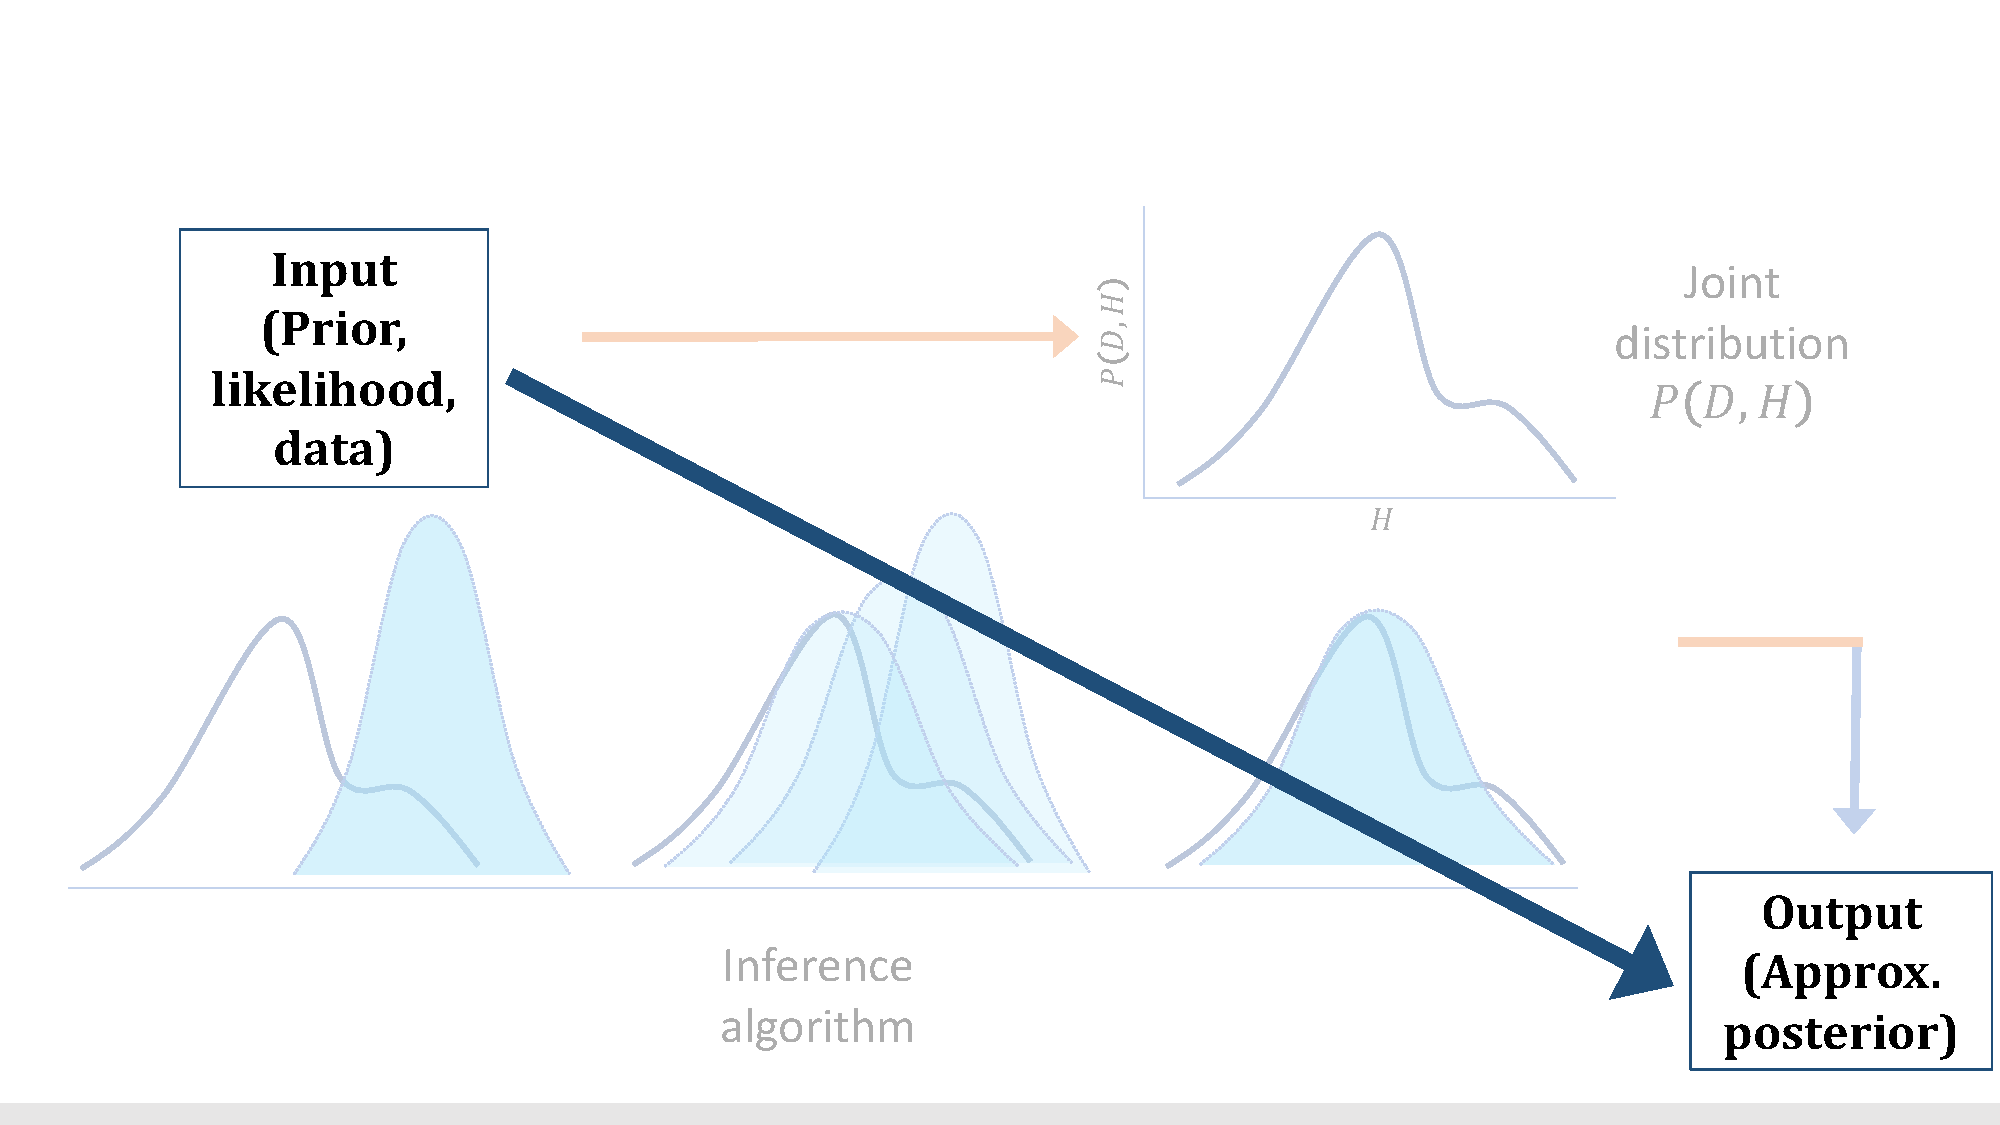
\includegraphics[width = \textwidth]{figures/var_schematic_amort.pdf}
\caption{\textbf{Schematic for Amortized Variational approximation}. }
\label{fig:var_schematic_amort}
\end{figure}

In a variational framework, the approximate posterior $\hat{P}(h | d)$ is a member of some parametrized family that we choose. These parameters therefore can be re-used from query to query. A key advantage of representing the approximate posterior as a finite set of variational parameters, rather than a variable number of random samples, is that it makes it easier to flexibly re-use inferences. I outline below how this might be possible.

In Figure \ref{fig:var_schematic}, we introduced a schematic for variational approximation. To better understand flexible re-use in this framework, we consider a variant of this schematic in Figure \ref{fig:var_schematic_amort}. The key observation here is that a variational approximation determines a mapping from inputs (priors, likelihoods and data) to the output (a posterior approximation). One path to go from the input to the output is to explicitly solve the variational problem. Over extensive experience in a domain, we will have solved this variational problem for a variety of inputs. Therefore, we have built up a large number of such input-output pairs. We are therefore in a position to see if there are any patterns in this mapping from input to output, that we can use to best inform future computations. This can be done by simply learning a regression function, from previous input-output pairs, that maps a query (data, prior, likelihood) to an output.\footnote{The inductive biases we use in the regression function that we learn will influence the outputs predicted for new inputs. See Chapter \ref{chap:LTI} for a more detailed discussion of this.} This gives us a second path to go from the inputs to outputs. When faced with a brand new query -- that is different from other faced before -- this mapping allows us to immediately have a guess for the approximate posterior, by simply passing the parameters of this new query through our learned regression function. This initial point can be further optimized using the standard optimization procedure used for variational inference, but will usually require fewer steps of optimization, and fewer computational resources, if our initial guess is well-informed (the learned mapping captures the right structure). In this way, we can use information gathered from previously computed input-output pairs to amortize the cost of finding variational approximations for new inputs. In Chapter \ref{chap:LTI}, we show that many errors and biases observed in human probabilistic judgment are explained by this mechanism.

Variational approximations still have the disadvantage that they have no asymptotic guarantees, while sampling methods do. A promising way forward is to combine the complementary advantages. Most Monte Carlo approximations rely on having a good `proposal distribution' that closely approximates the true posterior, in order to converge quickly and provide good approximate posterior probabilities under realistic limitations on the number of samples. We expect humans to be in this low sample regime when using Monte Carlo methods, due to the limitations imposed by their cognitive limitations. Variational approximations could provide this proposal distribution. This way, we can retain the flexible re-use permitted by variational inference, as well as the asymptotic guarantees of sampling. As we will see in Chapters \ref{chap:MCMC} and \ref{chap:LTI}, such a joint model allows us to parsimoniously explain a wide range of different inferential errors that could not be modeled by any one mechanism alone. This possibility is discussed in greater detail in Chapter \ref{chap:LTI} in Section \ref{sec:LTI_sampl_integ}.

\subsection{Amortization in discriminative machine learning}

In this section, we briefly discuss how `pattern-matching' methods popular in modern machine learning, can be seen as amortizing inference over past experience. We limit our discussion here to a simple case of discriminative classification. In the next section on amortization in cognitive science, we also discuss various reinforcement learning (RL) methods that are also popular in modern machine learning, and their interpretation as amortized inference.

The key difference between our discussion of amortization (in various approximate inference methods) so far and most realizations of amortization in machine learning, is that for many machine learning applications, the potential knowledge has not already been acquired, and is obtained in tandem with learning how to go from potential to realized knowledge. In other words, learning about the world, and learning how to think are not done separately. These are called discriminative methods; as opposed to generative methods that explicitly learn the generative model (potential knowledge) and then proceed with inference in that model (realized knowledge). Both these approaches (generative and discriminative) are ubiquitous in many machine learning with competing advantages for each\citep{ng2002discriminative, lasserre2006principled}.The machine learning methods we discuss in this thesis (in Chapters \ref{chap:sentences} and \ref{chap:causal}) are discriminative. We give a simple example of discriminative classification here, to give an intuition for how these methods can be interpreted as a form of amortization.

The basic classification problem is that of categorizing various inputs $\{x\}$ into various classes $\{y\}$. This can be seen as computing some probability distribution $P(y | x)$ i.e. the probability distribution over class labels given a specific input $x_i$, and then employing some decision rule to assign that input to different classes, based on the obtained distribution. \footnote{This is the key to a discriminative approach to classification. The generative approach to this problem would be to explicitly learn the generative model described by the joint distribution $P(x, y) = P(y) P(x | y)$, and subsequently use Bayes' rule to find $P(y | x)$.  Inference in such generative models can also be amortized, for example by using the approaches discussed earlier for amortization within approximate inference algorithms. } We can look at this as a multinomial (or binomial) posterior distribution over class labels, conditioned on the data, i.e. the features of of the input point $x$. The key difference between our previous discussions and this one, is that we do not know the joint distribution already, and therefore cannot `learn' this function by maximizing ELBO like we did in the variational case. Instead, a common approach is to learn it with supervision -- i.e. by receiving observations of the right classification, and maximizing the probability of the true class labels under our discriminative classifier. Discriminative classifiers can also be learned via reinforcement learning, as we will discuss briefly in the next section. The idea is that once this conditional distribution $P(y | x)$ has been learned over a series of training examples, this function can be used to predict the conditional distribution in new test examples, or new $x$s that have not been observed. This can be done with single pass through this learned regression from input to class label. In other words, the computations that would otherwise have gone into explicitly computing the posterior $P(y | x)$, had we known the joint $P(y,x)$ have been amortized, and have been encoded along with  the relevant potential knowledge about $P(y,x)$, in this discriminative function. This is similar to the amortized variational approximation we learn in the previous section, except the learning signal that we used to learn the function is different (supervised or reinforcement learned in this setting, as opposed to via maximization of ELBO). Such a supervised classifier underlies the artificial system we analyze in Chapter \ref{chap:sentences}.

\subsection{Meta-learning and amortization}
Meta-learning is a sub-field of machine learning where information is gained over a distribution of learning tasks about how to learn in new tasks from the same distribution. In other words, we can \textit{learn to learn} by abstracting out higher level in information about the space of learning tasks that benefit future learning. Many features of a learning algorithm can be `meta-learned' in this way, including the optimization algorithm to be used in new learning problems\citep{andrychowicz2016learning}, good initial weight parameters\citep{finn2017model}, the right metric space for gauging similarities\citep{vinyals2016matching}, as well the use of external memory\citep{santoro2016meta}.  In the same way that the discriminative methods discussed in the previous section blur the lines between gaining potential knowledge and converting potential to realized knowledge, meta-learning is agnostic to whether what it learns from its experience is new information about the world (learning about the underlying process that is generating the distribution of learning tasks), or how to make best use of information in a new learning task (faster, more efficient amortized inference strategies). Meta-learning has been characterized as hierarchical Bayesian inference, where what is being learned are abstract priors over the space of learning tasks, such that knowledge gained from solving one task can transfer to the learning of other tasks from the same distribution.\citep{ortega2019meta, grant2018recasting, griffiths2019doing} However, meta-learning methods usually also implicitly learn amortized inference strategies. We discuss in greater detail the distinction between these two kinds of learning in Chapter \ref{chap:conclusion}.

\section{Amortization in cognitive science}

It is an uncontroversial observation in cognitive science that experience in a certain domain and greater familiarity with it leads to easier, faster, almost automatic inferences. Amortization offers an explanation for this phenomena. As phrased by \citet{logan1988toward}:
\begin{quote}
``Automaticity is memory retrieval: Performance is automatic when it is based on single step direct-access retrieval of past solutions from memory. The theory assumes that novices begin with a general algorithm that is sufficient to perform the task. As they gain experience, they learn specific solutions to specific problems, which they retrieve when they encounter the same problems again.''
\end{quote}
Amortization formalizes this notion of flexible re-use of past computations, despite already having a `general algorithm sufficient to perform the task'. This allows faster, more automatic inferences with more experience.

This results in a dependence on the history of queries observed, leading to another key prediction of amortizing inference. If there is additional structure in this historical query set, we expect the development of ecologically rational shortcuts that reflect this structure. These shortcuts might give close to optimal responses on commonly observed queries, but would give poor performance on uncommon ones. This provides a potential explanation for some kinds of biased inference in humans. We will also see how this can inform inference procedures learned in artificial systems. Note that if computations were being carried out from scratch -- computing realized knowledge from potential knowledge each time -- there would be no difference in behavior between common and uncommon queries.

Here, I discuss how amortization has been an implicit part of many approaches in modeling human cognition, focusing in particular on two domains: Inference and planning. Planning can be seen as a specific case of inference\citep{botvinick2012planning}, but these have historically been studied as separate problems, with various approaches to each developing independently. %So we first address amortization in these two separately and then discuss how methods developed in each can inform one another, when seen through the common lens of amortization.

\subsection{Amortization in Inference}

%In the problem of exact Bayesian inference discussed in Chapter \ref{chap:approx}, the goal is to make a judgment about posterior probabilities $P(h | d)$.  From this potential knowledge, we can in theory then compute posterior probabilities (i.e. realized knowledge), but this step comes with the computational costs of performing exact or approximate posterior inference.

I first briefly reiterate the computational problem underlying Bayesian inference. In many real-world situations, people have to combine information from many sources, in order to make judgments about probabilistic outcomes. As discussed in Chapter \ref{chap:psych}, Bayesian inference provides a normative computational account of what should be done. The first step in Bayesian inference is acquiring the requisite potential knowledge  -- i.e. to collect information from the world in order to inform a joint distribution $P(h,d)$. This includes learning a prior distribution $P(h)$ as well as a likelihood function $P(d | h)$. We will assume that this step is already complete. The second step, that we focused on in Chapter \ref{chap:approx} is of going from the possible to realized knowledge. That is, of computing normalized posterior probabilities  $P(h |d)$. Given data $d$, Bayes' rule stipulates how a rational agent should update its prior probabilistic beliefs $P(h)$ about hypothesis $h$:
\begin{align}
    P(h|d) = \frac{P(d|h)P(h)}{\sum_{h'} P(d|h') P(h')},
\end{align}
where $P(h|d)$ is the agent's posterior distribution, expressing its updated beliefs. In case of many underlying hypotheses (as is often the case), this denominator is difficult and often intractable to calculate. Therefore, despite having the requisite `possible ' knowledge in the form of the generative model $P(h,d)$, the `realized' knowledge of the posterior probabilities are non-trivial and remain a computational challenge.

Amortization suggests that this computation be spread out over previously encountered queries. This suggests that greater experience in a domain, or practice in the domain, will lead to faster inferences. This has been found and studied extensively in the literature on practice\citep{gobet2001chunking, newell1981mechanisms} and automatic processing\citep{shiffrin1977controlled, logan1988toward}, even after there is no new information to be gained by increased experience. 

Further, the structure of queries often have a lot of underlying lower-dimensional structure, with certain kinds of queries being much more likely than others (despite all queries being equally answer-able based on existing potential knowledge). An amortized inference strategy will reflect this structure, as discussed previously, and could encode heuristics that hold only in the space of common queries, leading to biased inference. The use of heuristic-based strategies has been observed in experts in various domains such as legal decisions \citep{dhami2001bailing}, and medicine \citep{reyna2006physician}, where the most general, normative decision strategy involves several variables and is often too complex for easy full consideration. \cite{garcia2009take} find, in a domain of criminality and law enforcement, that expert behavior is better described by heuristic strategies, while laypeople are better described by a full regression to the relevant variables. These provide preliminary evidence that these heuristic strategies are in fact learned from experience, and amortization provides a mechanism for how these context-sensitive heuristics might arise.

%In thinking of a heuristic as a learned function from query to response, the role of memory becomes more obvious. Previous experience stored in memory, provides a set of input queries and output responses -- where the response was either computed using a noisy general purpose, normative strategy, or externally provided say by a teacher. These pairs can be used to fit a function, i.e. find a heuristic, that is separate from the normative decision strategy. Previous work \citep{gluck1988conditioning, dasgupta2019theory, shanks1991connectionist} has demonstrated that different approximate solutions to general-purpose probabilistic inference can arise from such a mapping, and that these vary depending on the distribution of queries. 

%Also integrates with episodic re-use of specific examples (connection to \cite{dasgupta2018remembrance}), by informing when to re-use (analogous to episodic RL, learning a similarity function).

\subsection{Amortization in Planning}

While the main focus of this paper is on inference and not planning, amortization has implicitly played a very crucial role in our understanding of how planning might be implemented. In this section, we briefly discuss the computational challenge of exact planning, and how amortization fits into the framework of approximate planning. We then discuss how these might inform our primary discussion on amortization in inference.

\subsection*{The planning problem}

The goal of planning is to leverage information one has about the world (realized knowledge) in order to achieve a specific goal (potential knowledge). Here as well, the main challenge is in the computations that go from potential to realized knowledge, This problem has been commonly studied in a Markov Decision Process paradigm, in the context of Reinforcement Learning (RL). The framework here is that an agent has a fixed set of actions ($a \in A$) it can perform on the world, in order to receive reward ($r$). This reward depends on both the state of the world the agent is in ($s \in S$) as well as the action taken, as defined by a reward function $r = R(s, a)$. The goal is to maximize this earned reward, over some fixed or discounted (by some factor $\gamma < 1$) time horizon. The effect of an action will depend on the state of the world the agent is in, and can cause a transition from one state $s$ to another state $s'$ as defined by a transition model $P(s' | s, a)$. A common assumption, that makes the problem more tractable, is that the transitions and reward structure are Markov -- i.e. that when taking action $a$ in state $s$, which state we transition to ($P(s' | s, a)$) as well as the reward earned ($R(s,a)$) depend only on the current state and current action and is independent of the history of any previous states or actions.


% In the most general form of the problem, the agent does not know which state it is in and must additionally infer the state it is in from observations O. If an observation does not uniquely identify the underlying state, then the Markov assumption no longer holds. The goal is to learn a policy i.e. a mapping from observations to action, that maximizes reward.

In a planning problem, the transition probabilities and reward functions are known -- this consists of all the potential knowledge about this domain. The challenge in converting this to realized knowledge is to construct a \textit{policy} $\pi: S \rightarrow A$ that determines what action to take at each state, in order to maximize the reward earned. The number of possible trajectories through the Markov Decision Process is exponentially large, and potentially infinite if there are cycles, and evaluating every possible policy -- despite already having all the potential knowledge in the domain -- is computationally very challenging and often entirely intractable. 

Amortization of previous computations, to better inform a policy, is a common approach to easing the burden of planning. The classic approach to this problem is to use dynamic programming or caching in the form of Bellman back-ups, where the expected reward associated with a state $s$, under a fixed policy $\pi$ is written as

\begin{equation}
V^{\pi}(s) = r(s) + \gamma \sum_{s' \in S} P(s' | s, \pi{s}) V^{\pi}(s')
\end{equation}

By writing the value of one state in terms of the value of another state, we can re-use the computations that went into computing these other values. These values can be computed iteratively with updating the policy, to find the optimal policy that maximizes reward using an algorithm called value-iteration. 

In cases where we might have a very large number of possible states, learning a table of these values becomes intractable. This includes most real-world relevant problems which in fact often have continuous state spaces. In these cases, we can learn a function that takes in properties of a state $s$ and returns its value $V(s)$. This way, even if the table of values actually computed (with dynamic programming in a known model) is sparse, and the values of other intermediate states are unknown, the function might be able to pick out (possibly heuristic) structure in the mapping from state to value. If this mapping is accurate, the function can generalize reasonably to new states without direct experience of that state. This is analogous to our discussion of amortization in a variational framework where `similar' queries can still benefit from computational re-use.

So far, we have only considered amortization as a solution to planning in a model in which the model is exactly known (model-based reinforcement learning). However, in many cases, the known model is either not known, or too complex to perform effective planning (even with help from dynamic programming). This is the broader reinforcement learning problem, where one must also obtain the relevant `potential knowledge' in terms of reward and transition structure, simultaneously with planning. In the absence of learning signals from planning in a known model, we can learn a value function directly from experience with the environment. Here, the learning signal from the model-based computed values is replaced with stochastic rewards actually experienced in the environment. This is often termed a model-free approach to reinforcement learning\footnote{This is a useful distinction and we follow this convention for the rest of the section. However, a calling a discriminative methods `model-free' can be misleading. It can instead be characterized as learning a simpler model that maps states to values. We expand on this interpretation in our discussion on simultaneous learning of model and inference in Chapter\ref{chap:conclusion}.}. A similar approach is often used to obtain not just state-specific values, but the value of state-action pairs in a process known as Q-learning\citep{watkins1992q}. Efficient algorithms for these model-free approaches to reinforcement learning, paired with the generalization and representational capacity of deep neural networks, underlie many recent successes in artificially intelligence\citep{mnih2013playing}, as well as underlies the artificial agent we analyze in Chapter \ref{chap:causal}. Here, potential and realized knowledge are not encoded separately and are simply learned end-to-end. This is therefore a discriminative approach, as discussed in the earlier section on amortization in machine learning.

\subsection*{Studies in cognitive science}

In cognitive science, amortized planning has largely been studied in the context of the larger reinforcement learning problem. Therefore, rather than as amortization within a model-based framework, it has largely been studied directly as model-free approaches to reinforcement learning. If we have the right model, and infinite experience to learn model-free values, then exact planning in a model, and the learned model-free values will correspond exactly. However, most studies of reinforcement learning and decision making in natural intelligence distinguish these kinds of learning by leveraging the fact that model-free values are very efficient once they have been learned but adapt very slowly to changes in reward structure and transition probabilities, whereas model-based inference is equally expensive with a new or an old transition / reward function\citep{daw2011model}. These are also distinguished based on the extent of cognitive effort required and available at run-time, with the logic that model-free values are habitual and automatic, requiring less processing than planning in a model\citep{otto2014cognitive, kool2017cost}. The neural realizations of these different learning systems have also been studied extensively\citep{glascher2010states, o2003temporal}. 
%Recent work has also worked to distinguish the real-time processes that these two learning mechanisms entail in the brain. 

To better draw parallels to our discussion of amortization in inference, we consider a hybrid between model-based and model-free systems, namely the DYNA architecture\citep{sutton1991dyna}. Here, the model is learned and stored i.e. all potential knowledge is explicitly acquired based on external experience. However, model-free values are not learned solely from interaction with the environment, and are instead updated using simulations in this model. Updating model-free values using model-based values is more analogous to our discussion of amortization in inference where the only computations being amortized in going from potential to realized knowledge. Evidence of DYNA-like behavior has also been found in humans\citep{gershman2014retrospective}.

Other approaches to reinforcement learning have also implicitly invoked amortization of planning. The successor representation\citep{dayan1993improving} is an ecological rational adaptation to worlds in which the transition function $P(s' | s, a)$ does not often change, but the reward function $R(s, a)$ does. This implicitly amortizes computations by re-using past experience of transition probabilities, but remains flexible on reward structure. Episodic approaches to reinforcement learning-- where the computational challenge is to learn similarity functions to previous experience, to facilitate adaptive re-use\citep{gershman2017reinforcement} -- can also be seen as amortization. Certain aspects of planning can also be meta-learned (see the earlier section on meta-learning for details), thereby amortizing some of its costs\citep{botvinick2019reinforcement}. In fact we will see in Chapter \ref{chap:causal}, how amortized model-free methods in a meta-learning framework can also lead to realizations of other more complex amortized inference procedures.

Amortized planning also has implications for the strategy selection problem discussed earlier in the context of domain-specific, ecologically rational heuristics. Choosing the right strategy has often been framed as meta-cognitive reinforcement learning problem. \cite{erev2005adaptation, rieskamp2006ssl, lieder2017strategy}. Here an agent operates in a `meta-cognitive Markov Decision Process' and decides how much information to gather, how much cognitive energy to invest, and what inference strategies to use, with the ultimate goal of optimizing a bounded rationality objective function that rewards good inferences and penalizes costs. Without further assumptions, optimal planning in this Markov Decision Process remains intractable, and amortized planning methods developed in reinforcement learning suggest possible solutions.

%Empirical evidence of such offline updating has been suggested and studied in the context of reinforcement learning via the DYNA architecture \citep{sutton1990integrated, gershman2014retrospective}, moral judgements via empathy-based appraisal \citep{ugazio2014empathy, van2016imaginative}, modal cognition via the evaluation of conditionals and counterfactuals \citep{ichikawa2012rational, phillips2018psychological, williamson2007philosophical, roese1997counterfactual}, and consolidation via replay (during sleep?, unsure if hippocampal reply can be characterized as `from a model' to a compiled response).

%The first is more flexible, since it allows one to predict the effects of actions in situations never previously encountered directly, and is quickly able to adapt its policy to changing reward structures. The second is less flexble since (in its most basic form), requires each observation-action pair to have been experienced in order to know its value. Further, if the reward structure changes, then all of these observation-action pairs need to be revisited in order to revise the new values of each of these. On the flip-side, the model-based strategy is very computationally expensive at run-time -- it requires the simulation of several steps into the future, and a combinatorially high number of possible trajectories to evaluate the value of an action. Whereas the model-free strategy uses previous experience in the domain to inform future the value of actions, and saves significant computational energy at run-time.

%The model-based representation is "potential knowledge" that is, it contains within it all the required information to maximize reward in the environment. However, compiling it into an actionable policy, is computationally expensive. The model-free representation however contains compiled knowledge that directly informs actionable policy, at the cost of throwing away the flexibility of abstraction. One way to integrate these advantages is to use a learned world model to perform planning in advance, and compile the results into rapidly recoverable query-response rules which can be easily used for real-time inference. This architecture is often referred to as DYNA, as was discussed briefly in the previous section. In this section, rather than overlaying these two approaches as with DYNA, we explore instead the continuum between these two diametrically opposite approaches. We investigate how various approaches to approximate planning can be seen as different points on an amortization spectrum. Here, the distinction between the two kinds of knowledge -- possible and compiled / realized -- is less clear since both have to be acquired. Instead we focus on how different frameworks trade-off abstraction (i.e. a flexible representation that encompasses all `possible' knowledge) and computational resources (i.e. a compiled response that represents `realized' knowledge and directly informs strategies). We outline how different points on this spectrum might be optimal for different environments, depending on the complexity of the world and the variability in the query distribution.

%Model-free value functions, pruning. Episodic RL. Temporal abstraction, options. Successor representation -- since much of the important structure in the environment is baked into the representation, simple computations with this representation can give good responses. 
%
%\subsection{A fruitful exchange}
%
%Our main interest in this thesis in finding ways to make Bayesian inference tractable. This detour into amortized planning and a review of its study in cognitive science highlight two crucial ways in which the study of amortized planning can be leveraged to better inform our study of amortization in inference.
%
%First, the strategy selection problem -- a central issue the study of domain-specific, ecologically rational heuristics as a solution to bounded rationality -- has often been framed as meta-cognitive reinforcement learning problem. \cite{erev2005adaptation, rieskamp2006ssl, lieder2017strategy}. Here, an agent decides not only the actions it wants to take in the outside world, but also decides how much information to gather, how much time to spend, as well as how much cognitive energy to invest, in improving an inference. This can be formalized as a meta-cognitive Markov Decision Process. However, without further assumptions, optimal planning in this Markov Decision Process remains a computational challenge, and is often intractable. Amortized planning methods developed in reinforcement learning suggest efficient solutions to this problem via the re-use of past experience, thereby suggesting feasible algorithmic solutions to ecologically rational inference. A key constraint in thThis could integrate with  this idea in Chapter \ref{chap:LTI}.
%
%Second, a meta-learning framework allows the learning of new inference strategies. We will show how amortized planning in a meta-reinforcement learning framework can give rise to new, sophisticated inference strategies, in Chapter \ref{chap:causal}.